\documentclass[tikz,border=12pt]{standalone}
\usepackage{tikz}
\usepackage{amsmath}
\usetikzlibrary{arrows.meta,fit,backgrounds}

%% P8 vs P9 key improvement comparison

\definecolor{cP8}   {RGB}{185, 45,  45}
\definecolor{cP9}   {RGB}{40,  145, 70}
\definecolor{cArrow}{RGB}{80,  80,  80}
\definecolor{cNote} {RGB}{80,  80,  80}
\definecolor{cFeat} {RGB}{60,  110, 200}
\definecolor{cGood} {RGB}{40,  145, 70}
\definecolor{cBad}  {RGB}{185, 45,  45}

\tikzset{
  B/.style    = {draw, thick, rounded corners=4pt, text centered,
                 font=\small, minimum height=11mm},
  p8B/.style  = {B, fill=cP8!12,  draw=cP8!70},
  p9B/.style  = {B, fill=cP9!12,  draw=cP9!70},
  inpB/.style = {B, fill=gray!10, draw=gray!55, minimum width=24mm},
  badB/.style = {B, fill=cBad!10, draw=cBad!55, minimum width=60mm,
                 font=\scriptsize},
  goodB/.style= {B, fill=cGood!10,draw=cGood!55, minimum width=60mm,
                 font=\scriptsize},
  note/.style = {draw=cNote!40, rounded corners=4pt, fill=gray!5,
                 font=\scriptsize, text=cNote, inner sep=6pt, align=left},
  A/.style    = {-Stealth, thick},
  Adash/.style= {-Stealth, dashed, thick, opacity=0.6},
}

\begin{document}
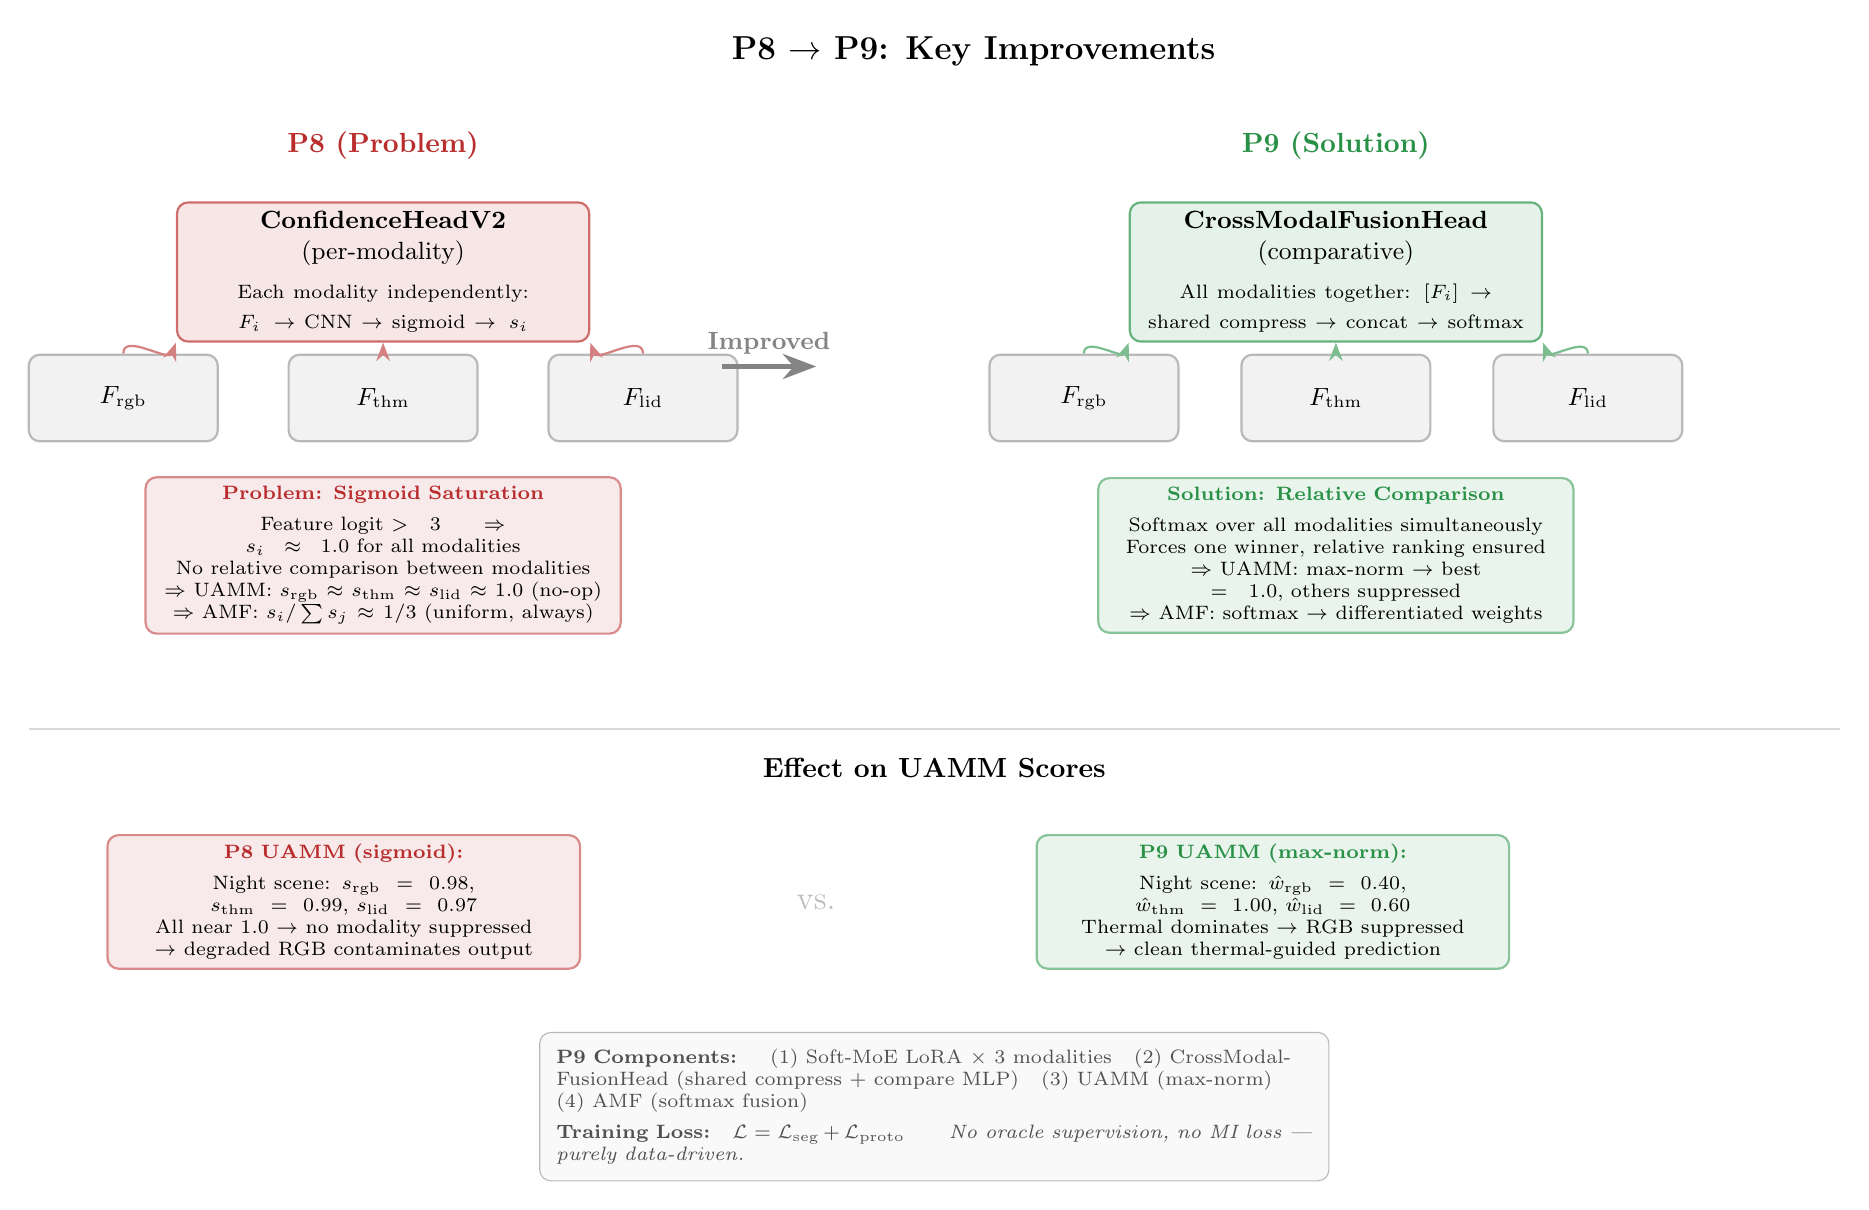
\begin{tikzpicture}

%% ─── Title ───────────────────────────────────────────────────────
\node[font=\large\bfseries, text=black] at (12.0, 1.0)
  {P8 $\to$ P9: Key Improvements};

%% ════════════════════════════════════════════
%%  LEFT: P8 (problem)
%% ════════════════════════════════════════════
\node[font=\normalsize\bfseries, text=cP8] at (4.5,-0.2) {P8 (Problem)};

%% P8 Confidence Head
\node[p8B, minimum width=52mm, minimum height=16mm, text width=50mm]
  (ch) at (4.5,-1.8)
  {\textbf{ConfidenceHeadV2} (per-modality)\\[3pt]
   {\scriptsize Each modality independently: $F_i \to$ CNN $\to$ sigmoid $\to s_i$}};

\node[inpB] (fR8) at (1.2,-3.4) {$F_\text{rgb}$};
\node[inpB] (fT8) at (4.5,-3.4) {$F_\text{thm}$};
\node[inpB] (fL8) at (7.8,-3.4) {$F_\text{lid}$};

\draw[A, cP8!60] (fR8.north) to[out=90,in=250] (ch.south west);
\draw[A, cP8!60] (fT8.north)--(ch.south);
\draw[A, cP8!60] (fL8.north) to[out=90,in=290] (ch.south east);

%% Problem: sigmoid saturation
\node[badB, text width=58mm] at (4.5,-5.4)
  {{\color{cBad}\textbf{Problem: Sigmoid Saturation}}\\[3pt]
   Feature logit $> 3 \;\Rightarrow\; s_i \approx 1.0$ for all modalities\\
   No relative comparison between modalities\\
   $\Rightarrow$ UAMM: $s_\text{rgb} \approx s_\text{thm} \approx s_\text{lid} \approx 1.0$ (no-op)\\
   $\Rightarrow$ AMF: $s_i / \sum s_j \approx 1/3$ (uniform, always)};

%% ─── Arrow from P8 to P9 ─────────────────────────────────────────
\draw[-Stealth, very thick, cArrow!70, line width=2pt]
  (8.8,-3.0) -- node[above, font=\small\bfseries]{Improved} (10.0,-3.0);

%% ════════════════════════════════════════════
%%  RIGHT: P9 (solution)
%% ════════════════════════════════════════════
\node[font=\normalsize\bfseries, text=cP9] at (16.6,-0.2) {P9 (Solution)};

%% P9 CrossModalFusionHead
\node[p9B, minimum width=52mm, minimum height=16mm, text width=50mm]
  (cmf) at (16.6,-1.8)
  {\textbf{CrossModalFusionHead} (comparative)\\[3pt]
   {\scriptsize All modalities together: $[F_i] \to$ shared compress $\to$ concat $\to$ softmax}};

\node[inpB] (fR9) at (13.4,-3.4) {$F_\text{rgb}$};
\node[inpB] (fT9) at (16.6,-3.4) {$F_\text{thm}$};
\node[inpB] (fL9) at (19.8,-3.4) {$F_\text{lid}$};

\draw[A, cP9!60] (fR9.north) to[out=90,in=250] (cmf.south west);
\draw[A, cP9!60] (fT9.north)--(cmf.south);
\draw[A, cP9!60] (fL9.north) to[out=90,in=290] (cmf.south east);

%% Solution: relative comparison
\node[goodB, text width=58mm] at (16.6,-5.4)
  {{\color{cGood}\textbf{Solution: Relative Comparison}}\\[3pt]
   Softmax over all modalities simultaneously\\
   Forces one winner, relative ranking ensured\\
   $\Rightarrow$ UAMM: max-norm $\to$ best $= 1.0$, others suppressed\\
   $\Rightarrow$ AMF: softmax $\to$ differentiated weights};

%% ════════════════════════════════════════════
%%  BOTTOM: P8 vs P9 UAMM comparison
%% ════════════════════════════════════════════
\draw[gray!30, thick] (0,-7.6)--(23.0,-7.6);

\node[font=\normalsize\bfseries] at (11.5,-8.1) {Effect on UAMM Scores};

%% P8 UAMM
\node[badB, text width=50mm] at (4.0,-9.8)
  {{\color{cBad}\textbf{P8 UAMM (sigmoid):}}\\[3pt]
   Night scene: $s_\text{rgb}=0.98$, $s_\text{thm}=0.99$, $s_\text{lid}=0.97$\\
   All near 1.0 $\to$ no modality suppressed\\
   $\to$ degraded RGB contaminates output};

%% P9 UAMM
\node[goodB, text width=50mm] at (15.8,-9.8)
  {{\color{cGood}\textbf{P9 UAMM (max-norm):}}\\[3pt]
   Night scene: $\hat{w}_\text{rgb}=0.40$, $\hat{w}_\text{thm}=1.00$, $\hat{w}_\text{lid}=0.60$\\
   Thermal dominates $\to$ RGB suppressed\\
   $\to$ clean thermal-guided prediction};

\node[font=\large, text=gray!50] at (10.0,-9.8) {vs.};

%% ─── Summary note ────────────────────────────────────────────────
\node[note, text width=96mm] at (11.5,-12.4)
  {\textbf{P9 Components:}
   \quad (1) Soft-MoE LoRA $\times$ 3 modalities\quad
   (2) CrossModalFusionHead (shared compress + compare MLP)\quad
   (3) UAMM (max-norm)\quad
   (4) AMF (softmax fusion)\\[3pt]
   \textbf{Training Loss:}\quad
   $\mathcal{L} = \mathcal{L}_\text{seg} + \mathcal{L}_\text{proto}$\qquad
   {\itshape No oracle supervision, no MI loss --- purely data-driven.}};

\end{tikzpicture}
\end{document}
